\chapter{Renewal Theory}
\label{ren}

\section{Introduction to Confidence Intervals}

\subsection{Example}

\label{bus}

Recall from our earlier unit the Bus Paradox:  Buses arrive at a certain
bus stop at random times, with interarrival times being independent
exponentially distributed random variables with mean 10 minutes.  You
arrive at the bus stop every day at a certain time, say four hours (240
minutes) after the buses start their morning run.  What is your mean
wait for the next bus?  We found that it is 10, but suppose we didn't
know that, and wished to find the answer via simulation.  We could write
a program:

\begin{Verbatim}[fontsize=\relsize{-2},numbers=left]
# Bus.py, illustration of the bus paradox

import random,sys

rnd = random.Random(12345)

def doexpt(opt):
   arvtm = 0.0
   while arvtm < opt:
      arvtm += rnd.expovariate(0.1)
   return arvtm-opt

def main():
   observationpoint = float(sys.argv[1])
   nreps = int(sys.argv[2])
   sum = 0.0
   for i in range(nreps):
      wait = doexpt(observationpoint)
      sum += wait
   print 'the estimated mean wait is', sum/nreps

if __name__ == '__main__': main()
\end{Verbatim}

Running the program yields

\begin{Verbatim}[fontsize=\relsize{-2}]
% python Bus.py 240 1000
the estimated mean wait is 10.2182290246
\end{Verbatim}

Was 1000 iterations enough?  How close is this value 10.2182290246 to
the true expected value of waiting time?\footnote{Of course, continue to
ignore the fact that we know that this value is 10.0.  What we're trying
to do here is figure out how to answer ``how close is it'' questions 
in general, when we don't know the true mean.}

What we would like to do is something like what the pollsters do during
presidential elections, when they say ``Ms. X is supported by 62\% of
the voters, with a margin of error of 4\%.''  In fact, we will do
exactly this, in the next section.

\subsection{Confidence Intervals for Means}
\label{cim}

In our example in Section \ref{bus}, let $W$ denote the random wait
time one experiences in general in this situation.  We are using the
program to estimate $E(W)$, which we will denote by $\mu$.  While we're
at it, let's denote $Var(W)$ by $\sigma^2$.

Before we go on, it's important that you first recall what EW and Var(W)
really mean, say via our ``notebook'' view.  We come to the bus stop
every day at the same time, and each day we would record our waiting
time on a separate line of the notebook.  EW and Var(W) would mean the
mean and the variance of all the values of W we record (technically
after an infinite number of days).  Similarly, $F_W(12.2)$, for
instance, would mean the long-run proportion of notebook lines in which
$W \leq 12.2$.

\checkpoint

Let $W_i$ denote the $i^{th}$ waiting time, i = 1,2,... and let
$\bar{W}$ denote the sample mean,

\begin{equation}
\bar{W} = \frac{W_1+...W_n}{n}
\end{equation}

$\bar{W}$ is what the program prints out, and $n$ is our program's
variable {\bf nreps}. 

The key points are that

\begin{itemize}

\item the random variables $W_i$ have the distribution $F_W$

\item the random variables $W_i$ are independent

\item the mean of $\bar{W}$ is also $\mu$:

\begin{equation}
E(\bar{W}) = \frac{1}{n} \sum_{1}^{n} EW_i = \frac{1}{n} n \mu = \mu
\end{equation}

\item the variance of $\bar{W}$ is 1/n of the population variance:

\begin{equation}
Var(\bar{W}) = \frac{1}{n^2} \sum_{1}^{n} Var(W_i) = \frac{1}{n^2} n
\sigma^2 = \frac{1}{n} \sigma^2
\end{equation}

These points are indeed key, forming the very basis of statistics.

\checkpoint

\end{itemize}

The Central Limit Theorem then says that

\begin{equation}
Z = \frac{\bar{W}-\mu}{\sigma/\sqrt{n}}
\end{equation}

has an approximately N(0,1) distribution.  The tables for that
distribution tell us that 95\% of its area is between -1.96 and 1.96.
Thus

\begin{equation}
0.95 \approx P \left (-1.96 <  \frac{\bar{W}-\mu}{\sigma/n} < 1.96 \right )
\end{equation}

Doing a bit of algebra on the inequalities yields

\begin{equation}
\label{preci}
0.95 \approx P \left ( \bar{W} - 1.96 \frac{\sigma}{\sqrt{n}} < \mu
< \bar{W} + 1.96 \frac{\sigma}{\sqrt{n}} \right )
\end{equation}

Now remember, not only do we not know $\mu$, we also don't know
$\sigma$.  But we can estimate it, as follows:

Recall that by definition

\begin{equation}
\sigma^2 = E[(W-\mu)^2]
\end{equation}

Let's estimate $\sigma^2$ by taking sample analogs.  The sample analog
of $\mu$ is $\bar{W}$.  What about the sample analog of the ``E()''?
Well, since E() averaging over the whole population of Ws, the sample
analog is averaging over the sample.  So, we get

\begin{equation}
\label{s2}
\frac{1}{n} \sum_{i=1}^{n} (W_i-\bar{W})^2 
\end{equation}

In other words, just as it is natural to estimate the population mean of
W by its sample mean, the same holds for Var(W):

\begin{quote}
The population variance of W is the mean squared distance from W to its
population mean.  Therefore it is natural to estimate Var(W) by the
average squared distance of W from its sample mean, among our sample
values $W_i$.
\end{quote}

We $s^2$ as our symbol for this estimate of population
variance.\footnote{Though I try to stick to the convention of using only
capital letters to denote random variables, it is conventional to use
lower case in this instance.}

We will thus take our estimate of $\sigma$ to be $s$, the square root of
that quantity.

By the way, (\ref{s2}) is equal to 

\begin{equation}
\label{alts2}
s^2 = \frac{1}{n} \sum_{i=1}^{n} W_i^2 - \bar{W}^2
\end{equation}

However, this way of computing $s^2$ is subject to more roundoff error.

One can show that (\ref{preci}) is still valid if we substitute $s$ for
$\sigma$, i.e.

\begin{equation}
0.95 \approx P \left ( \bar{W} - 1.96 \frac{s}{\sqrt{n}} < \mu
< \bar{W} + 1.96 \frac{s}{\sqrt{n}} \right ) 
\end{equation}

In other words, we are about 95\% sure that the interval 

\begin{equation}
\label{meanci}
(\bar{W} - 1.96 \frac{s}{\sqrt{n}}, \bar{W} + 1.96 \frac{s}{\sqrt{n}})
\end{equation}

contains $\mu$.  This is called a 95\% {\bf confidence interval} for $\mu$.

We could add this feature to our program:

\begin{Verbatim}[fontsize=\relsize{-2},numbers=left]
# Bus2.py, illustration of the bus paradox

import random,sys
from math import sqrt

rnd = random.Random(12345)

def doexpt(opt):
   arvtm = 0.0
   nbus = 0
   while arvtm < opt:
      nbus += 1
      arvtm += rnd.expovariate(0.1)
   return arvtm-opt

def main():
   observationpoint = float(sys.argv[1])
   nreps = int(sys.argv[2])
   sum = 0.0
   sum2 = 0.0
   for i in range(nreps):
      wait = doexpt(observationpoint)
      sum += wait
      sum2 += wait**2
   wbar = sum/nreps
   wbar2 = sum2/nreps
   s = sqrt(wbar2-wbar**2)
   print 'the estimated mean wait is', wbar
   print 'with a 95% margin of error of', 1.96*s/sqrt(nreps)

if __name__ == '__main__': main()
\end{Verbatim}

In our example above, the interval would work out to (9.58,10.85).  We
would then say, ``We are about 95\% confident that the true mean wait
time until the next bus is between 9.58 and 10.85.''

{\bf What does this really mean?}  This question is of the utmost
importance.  We will devote the next section to it.

\subsection{Meaning of Confidence Intervals}

\subsubsection{A Weight Survey in Davis}

Consider the question of measuring the mean weight of all adults in the
city of Davis.  Say we sample 1000 people at random, and record their
weights, with $W_i$ being the weight of the $i^{th}$ person in our
sample.\footnote{Do you like our statistical pun here?  Typically an
example like this would concern people's heights, not weights.  But it
would be nice to use the same letter for random variables as in Section
\ref{cim}, i.e. the letter W, so we'll have our example involve peoples
weights instead of heights.  It works out neatly, because the word {\it
weight} has the same sound as {\it wait}.}

Say our interval turns out to be (142.6,158.8).  We say that we are
about 95\% confident that the mean weight $\mu$ of all adults in Davis
is contained in this interval.  {\bf What does this mean?}  Say we were
to perform this experiment many, many times:  We'd sample 1000 people at
random, then record our interval $(\bar{W} - 1.96 \frac{s}{\sqrt{n}},
\bar{W} + 1.96 \frac{s}{\sqrt{n}})$; then we'd sample another 1000
people at random, and record what interval we got that time (it would
have a different center and a different radius); then we'd do this a
third time, a fourth, a fifth and so on.  We would get a large number of
intervals---and approximately 95\% of them would contain $\mu$, the mean
weight in the entire adult population of Davis.

\checkpoint

It is customary to call $\bar{W}$ the {\bf sample mean}, as it is the
average value of W in our sample, and to call $\mu$ the {\bf population
mean}, as as it is the average value of W in the entire population.

Well, in our simulation case, it is {\it exactly the same situation}.
Simulation is a sampling process.  Our $\mu$ is the mean in the
``population'' of all bus waits, while $\bar{W}$ is the mean in our
sample of 1000 waits.  This is not mere analogy; mathematically the two
situations are completely identical.

Let's now admit that we actually know that from previous theory that $\mu$
is 10.  Then another way to see how to interpret confidence intervals is
to say that the output of the following program should be about 0.95:

\begin{Verbatim}[fontsize=\relsize{-2},numbers=left]
# Bus3.py, illustration of the bus paradox

import random,sys
from math import sqrt

rnd = random.Random(12345)

def doexpt(opt):
   arvtm = 0.0
   nbus = 0
   while arvtm < opt:
      nbus += 1
      arvtm += rnd.expovariate(0.1)
   return arvtm-opt

def main():
   observationpoint = float(sys.argv[1])
   nreps = int(sys.argv[2])
   count = 0
   for i in range(10000):
      sum = 0.0
      sum2 = 0.0
      for i in range(nreps):
         wait = doexpt(observationpoint)
         sum += wait
         sum2 += wait**2
      wbar = sum/nreps
      wbar2 = sum2/nreps
      s = sqrt(wbar2-wbar**2)
      if abs(wbar-10.0) < 1.96*s/sqrt(nreps): count += 1
   print count/10000.0

if __name__ == '__main__': main()
\end{Verbatim}

In fact, the output of that program was 0.9483, sure enough about
95\%.

\checkpoint

Why is it not exactly 0.95?  Well, first of all, we only did 10000
intervals.  But second, remember, the Central Limit Theorem itself is
only approximate, though for n = 1000 here it should be quite close.

\subsection{Why Not Divide by n-1?  And What About the Student-t
Distribution?}

It should be noted that it is customary in (\ref{s2}) to divide by n-1
instead of n, for reasons that are largely theoretical.  The reason for
this is that if we divide by n, as we have, then

\begin{equation}
\label{s2biased}
E(s^2) = \frac{n-1}{n} \cdot \sigma^2
\end{equation}

Let's prove (\ref{s2biased}).  We'll use (\ref{alts2}).  As before, let W
be a random variable distributed as the population.  Write

\begin{equation}
E(\sum_{i=1}^n W_i^2) = n E(W^2) = n[Var(W)+(EW)^2] =
n[\sigma^2 + \mu^2]
\end{equation}

\begin{equation}
E[\bar{W}^2] = Var(\bar{W}) + [E(\bar{W})]^2 = \frac{1}{n} \sigma^2 +
\mu^2
\end{equation}

Now using all this in (\ref{alts2}), we get

\begin{equation}
E(s^2) = \frac{n-1}{n} \sigma^2
\end{equation}

\checkpoint

In other words, the average value of $s^2$, over all possible samples,
is slightly smaller than $\sigma^2$.  We say that $s^2$ is {\bf biased},
with the amount of bias being

\begin{equation}
E(s^2) = \frac{1}{n} \cdot \sigma^2
\end{equation}

The earlier developers of statistics were bothered by this, so they
introduced a ``fudge factor'' by dividing by n-1 instead of n.

But when n is large---which is what we are assuming by using the Central
Limit Theorem---it doesn't make any appreciable difference.  

Moreover, speaking generally now rather than necessarily for the case of
$s^2$ there is no particular reason to insist that an estimator be
unbiased anyway, in general.  An alternative estimator may have a little
bias but much smaller variance, and thus be preferable.

\subsection{One More Point About Interpretation}

Some statistics instructors give students the odd warning, ``You can't
say that the probability is 95\% that $\mu$ is IN the interval; you can
only say that the probability is 95\% confident that the interval
CONTAINS $\mu$.'' This of course is nonsense.  Of course saying $\mu$ is
in the interval is equivalent to saying that the inteval contains $\mu$!

Where did this craziness come from?  Well, way back in the early days of
statistics, some instructor was afraid that a statement like ``The
probability is 95\% that $\mu$ is in the interval'' would make it sound
like $\mu$ is a random variable.  That was a legitimate fear, because
$\mu$ is not a random variable.  The random entity is the interval, not
$\mu$.  This is clear in our program {\bf Bus3.py} above---the 10 is
constant, while {\bf wbar} and {\bf s} vary from interval to interval.  

So, it was reasonable for teachers to warn students not to think $\mu$
is a random variable.  But later on, some statistics teachers just used
it as an unthinking rule, not understanding what the original concern
was, and as a result made foolish statements.

\subsection{Confidence Intervals for Proportions}
\label{propcis}

In our bus example above, suppose we also want our simulation to print
out the (estimated) probability that one must wait longer than 6.2
minutes:

\begin{Verbatim}[fontsize=\relsize{-2},numbers=left]
# Bus4.py, illustration of the bus paradox

import random,sys
from math import sqrt

rnd = random.Random(12345)

def doexpt(opt):
   arvtm = 0.0
   nbus = 0
   while arvtm < opt:
      nbus += 1
      arvtm += rnd.expovariate(0.1)
   return arvtm-opt

def main():
   observationpoint = float(sys.argv[1])
   nreps = int(sys.argv[2])
   sum = 0.0
   sum2 = 0.0
   gt62 = 0  # count of the number of waits > 6.2 minutes
   for i in range(nreps):
      wait = doexpt(observationpoint)
      sum += wait
      sum2 += wait**2
      if wait > 6.2: gt62 += 1
   wbar = sum/nreps
   wbar2 = sum2/nreps
   s = sqrt(wbar2-wbar**2)
   print 'the estimated mean wait is', wbar
   print 'with a 95% margin of error of', 1.96*s/sqrt(nreps)
   p62 = float(gt62)/nreps
   print 'the estimated probability of waiting longer than 6.2 is', p62

if __name__ == '__main__': main()
\end{Verbatim}

The value printed out for the probability is 0.544.  We again ask the
question, how can we determine how close this is to the true population
probability?

It turns out that we already have our answer, because a probability is
just a special case of a mean.  To see this, let

\begin{equation}
Y =
\begin{cases}
   1, & \text{if $W > 6.2$} \\
   0, & \text{otherwise} \\
\end{cases}
\end{equation}

Then

\begin{equation}
E(Y) = 1 \cdot P(Y = 1) + 0 \cdot P(Y = 0) = P(W > 6.2)
\end{equation}

Let $p$ denote this probability, and let $\hat{p}$ denote our estimate
of it; $\hat{p}$ is our {\bf p62} in the program.\footnote{The quantity
is pronounced ``p-hat.''  The ``hat'' symbol is traditional for
``estimate of.''}  Then a little algebra shows that

\begin{equation}
s^2 = \hat{p} (1-\hat{p})
\end{equation}

Equation (\ref{meanci}) becomes

\begin{equation}
\label{propci}
\left ( 
\hat{p} 
- 1.96 \sqrt{\hat{p} (1-\hat{p})/n},
\hat{p}
+ 1.96 \sqrt{\hat{p} (1-\hat{p})/n}
\right ) 
\end{equation}

We incorporate that into our program:

\begin{Verbatim}[fontsize=\relsize{-2},numbers=left]
# Bus5.py, illustration of the bus paradox

import random,sys
from math import sqrt

rnd = random.Random(12345)

def doexpt(opt):
   arvtm = 0.0
   nbus = 0
   while arvtm < opt:
      nbus += 1
      arvtm += rnd.expovariate(0.1)
   return arvtm-opt

def main():
   observationpoint = float(sys.argv[1])
   nreps = int(sys.argv[2])
   sum = 0.0
   sum2 = 0.0
   gt62 = 0  # count of the number of waits > 6.2 minutes
   for i in range(nreps):
      wait = doexpt(observationpoint)
      sum += wait
      sum2 += wait**2
      if wait > 6.2: gt62 += 1
   wbar = sum/nreps
   wbar2 = sum2/nreps
   s = sqrt(wbar2-wbar**2)
   print 'the estimated mean wait is', wbar
   print 'with a 95% margin of error of', 1.96*s/sqrt(nreps)
   p62 = float(gt62)/nreps
   print 'the estimated probability of waiting longer than 6.2 is', p62
   perr = 1.96*sqrt(p62*(1-p62)/nreps)
   print 'with a 95% margin of error of', perr

if __name__ == '__main__': main()
\end{Verbatim}

In this case, we get an interval of (0.51,0.57).

Note again that this uses the same principles as our Davis weights
example.  Suppose we were interested in estimating the proportion of
adults in Davis who weigh more than 150 pounds.  Suppose that proportion
is 0.45 in our sample of 1000 people.  This would be our estimate
$\hat{p}$ for the population proportion $p$, and an approximate 95\%
confident interval (\ref{propci})for the population proportion would be
(0.42,0.48).

Note also that although we've used the word {\it proportion} in the
Davis weights example instead of {\it probability}, they are the same.
If I choose an adult at random from the population, the probability that
his/her weight is more than 150 is equal to the proportion of adults in
the population who have weights of more than 150.

And the same principles are used in opinion polls during presidential
elections.  Here $p$ is the proportion of people who plan to vote for
the given candidate.  We again use (\ref{propci}).

Note that in both the Davis and election examples, it doesn't matter
what the size of the population is.  The distribution of $\hat{p}$, and
thus the accuracy of $\hat{p}$, depends only on $p$ and $n$, the latter
being the number of people we sample.\footnote{Implicit in our
assumption that the $W_i$ are independent is that we are sampling {\bf
with replacement}, which means it's possible that our random sampling
process might choose the same person twice.  But except for cases in
which our sample size is a substantial fraction of the population size,
the probability of getting the same person twice would be very low, so
it doesn't matter.} So if you've ever wondered how a nationwide election
poll can get by with sampling only 1200 people, which is a common
number, you now know the answer.

In fact, since the maximum possible value of $\hat{p} (1-\hat{p})$ is
0.25,\footnote{Use calculus to find the maximum value of f(x) = x(1-x).}
the pollsters know that their margin of error with n = 1200 will be at
most $1.96 \times 0.5/\sqrt{1200}$, or about 3\%. 

\subsection{Confidence Intervals for Differences of Means or Proportions}

\subsection{The Delta Method:  Confidence Intervals for General
Functions of Means or Proportions}

\subsection{Simultaneous Confidence Intervals} 

\subsection{Conditional Confidence Intervals}

Often in simulations we will be interested in conditional quantities.
In a queuing model, for instance, we might wish to estimate
the mean wait time of jobs which arrive when the server is busy.
We still use the usual formulas, e.g. (\ref{meanci}) and (\ref{propci}),
but keep in mind that the value of n in those formulas, even though we
might have run the simulation for a long time and the n for
unconditional quantities would be large.

\section{Estimation of Functions}

\subsection{Regression Analysis}

\subsubsection{Introduction}
\label{regintro}

Consider the Davis city population example again.  In addition to the
random variable $W$ for weight, let $H$ denote the person's height.
Suppose we are interested in exploring the relationship between height
and weight.

As usual, we must first ask, {\bf what does that really mean}?  What do
we mean by ``relationship''?  Clearly, there is no exact relationship;
for instance, we cannot exactly predict a person's weight from his/her
height.

Intuitively, though, we would guess that mean weight increases with
height.  To state this precisely, define

\begin{equation}
m_{W;H}(t) = E(W|H = t)
\end{equation}

This looks abstract, but it is just common-sense stuff.  For example,
$m_{W;H}(68)$ would be the mean weight of all people in the population
of height 68 inches.  The value of $m_{W;H}(t)$ varies with t, and we
would expect that a graph of it would show an increasing trend with t,
reflecting that taller people tend to be heavier.  

We call $m_{W;H}$ the {\bf regression function of W on H}.  In general,
$m_{Y;X}(t)$ means the mean of $Y$ among all units in the population for
which $X = t$.  Note that $X$ and t could be vector-valued.  For
instance, we could have $Y$ be weight and have $X$ be the pair (height,
age), so as to study the relationship of weight with height and age.

Now, let's again suppose we have a random sample of 1000 people from
Davis, with $(H_1,W_1),...,(H_{1000},W_{1000})$ being their heights and
weights.  We again wish to use this data to estimate population values.
But the difference here is that we are estimating a whole function now,
the whole curve.  That means we are estimating infinitely many values,
with one $m_{W;H}(t)$ value for each t.  How do we do this?

The traditional way is to make the simplifying assumption that $m_{W;H}(t)$
is a linear function of t, i.e.

\begin{equation}
\label{par}
m_{W;H}(t) = ct+d
\end{equation}

for some constants c and d.  If this assumption is reasonable---meaning
that though it may not be exactly true it is reasonably close---then it
is a huge gain for us.  Do you see why?  The answer is that instead of
having to estimate an infinite number of quantities, we now must
estimate only two {\bf parameters}---c and d.  Equation (\ref{par}) is
thus called a {\bf parametric} model of $m_{W;H}()$.

On the other hand, the linearity assumption may not be reasonable (there
are ways to assess this), in which case we would need a more general way
to estimate the function $m_{W;H}()$.  We'll discuss both ways below.

Before we do, though, we need to point out that the function $m_{W;H}$
makes sense even if $H$ is nonrandom.  To illustrate that, recall the
ALOHA network example from our introductory unit on simulation
(\url{http://heather.cs.ucdavis.edu/~matloff/156/PLN/SimIntro.pdf}).

I've adapted that a bit below:

\begin{Verbatim}[fontsize=\relsize{-2},numbers=left]
# AlohaC.py, form of slotted ALOHA

# here we will look finite time, finding the expected number of
# active nodes at epoch 8

# we'll run the simulation for many values of the backoff parameter b,
# to investigate the role b plays

import random, sys 

class node:  # one object of this class models one network node
   s = 4  # number of nodes
   b = None  # backoff parameter; refrain from sending with probability b
   q = 0.2  # msg creation probability
   activeset = []  # which nodes are active now
   inactiveset = []  # which nodes are inactive now
   r = random.Random(98765)  
   def __init__(self):  
      node.inactiveset.append(self)
   def checkgoactive():  # generate nodes which change to active
      for n in node.inactiveset:
         if node.r.uniform(0,1) < node.q:
            node.inactiveset.remove(n)
            node.activeset.append(n)
   checkgoactive = staticmethod(checkgoactive)  
   def trysend():  # the active nodes try to send, or not
      numnodestried = 0  
      whotriedlast = None  
      for n in node.activeset:
         if node.r.uniform(0,1) < node.b1:
            whotriedlast = n
            numnodestried += 1
      if numnodestried == 1:
         node.activeset.remove(whotriedlast)
         node.inactiveset.append(whotriedlast)
   trysend = staticmethod(trysend)  
   def reset():  
      for n in node.activeset:
         node.activeset.remove(n)
         node.inactiveset.append(n)
   reset = staticmethod(reset)  
            
def main():
   for i in range(node.s): node()
   bavg = []  # list of (b,avg) pairs
   nb = 100
   for i in range(nb):  # run for grid of b values
      node.b = float(i)/nb
      node.b1 = 1 - node.b
      sum = 0  # running total of active nodes at time 8
      for rep in range(1000):  # for fixed b, simulate 1000 times
         for epoch in range(8):  # simulate for 8 units of time
            node.checkgoactive()
            node.trysend()
         sum += len(node.activeset) 
         node.reset()
      bavg.append((node.b,sum/1000.0))
   for x,y in bavg:
      print x,y  # redirect this output to a file

if __name__ == '__main__': main()
\end{Verbatim}

A minor change is that I replaced the probability {\bf p} from before to 
{\bf b}, the probability of {\it not} sending.  The main change is that
I've added an extra outer loop, so as to try many values of {\bf b}.
Also, the output here is the mean number of active nodes at time 8,
which I'll call $A$ here.

I used the R statistical language\footnote{See \url{www.r-project.org}.
I have a quick tutorial on R at
\url{http://heather.cs.ucdavis.edu/~matloff/r.html}.} to plot $A$
against {\bf b}, seen in Figure \ref{scatter}. 

\begin{figure}[tb]
\centerline{
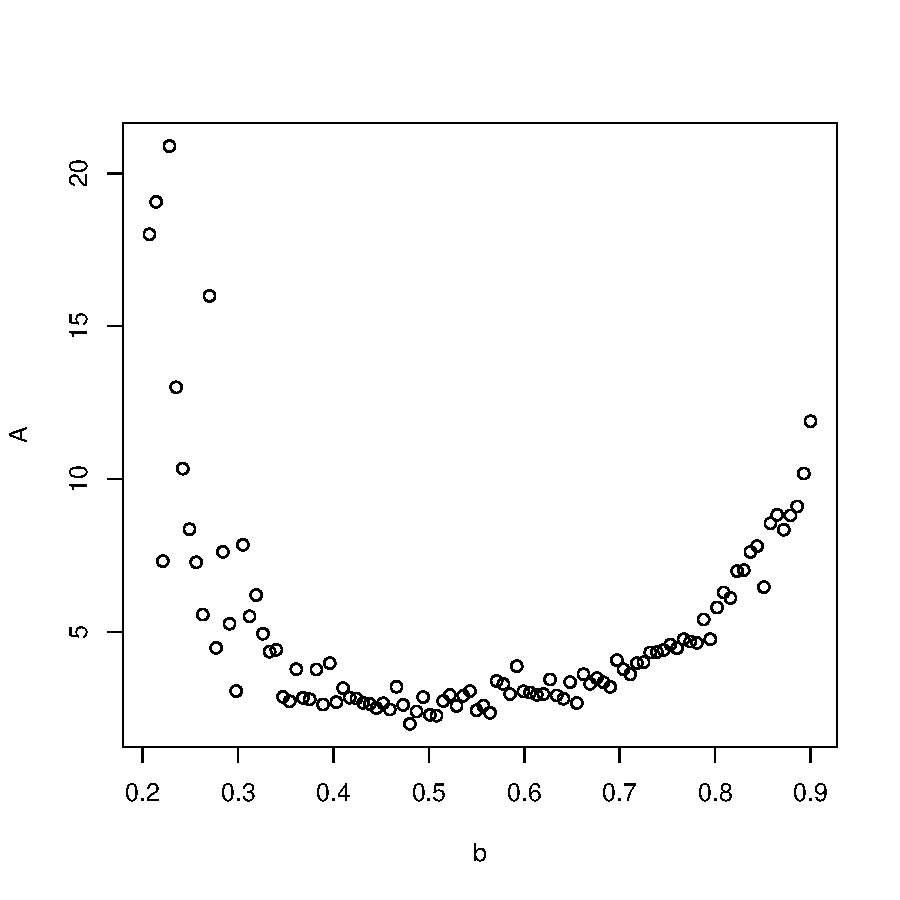
\includegraphics[width=5.0in]{Aloha1.pdf}
}
\caption{Scatter Plot}
\label{scatter}
\end{figure}


We do expect some kind of U-shaped relation, as seen here here.  For
{\bf b} too small, the nodes are clashing with each other a lot, thus
resulting in too many of them active when they should have already sent
out their data.  For {\bf b} too large, we are needlessly backing off in
many cases in which we actually would go through.

This looks like a quadratic relationship, or better stated, it looks
like  

\begin{equation}
\label{quad}
m_{A,b}(t) = \alpha_0 + \alpha_1 t + \alpha_2 t^2
\end{equation}

for some constants $\alpha_0, \alpha_1, \alpha_2$.  No model is exact,
but our data seem to indicate that this one is reasonably good, and if
further investigation confirms that, it provides for a nice compact
summary of the situation.  

We could then try other values of {\bf q}, and see how the quadratic curve
shifts, etc.  

So regression analysis makes sense even though $b$ is not a random variable.

\subsubsection{Parametric Estimation of Regression Functions}

Keep in mind that in (\ref{quad}), the $\alpha_i$ are population values.
We need to estimate them from our data.  Let's define $(b_i,A_i)$ to be
the $i^{th}$ pair from the simulation.\footnote{In the program, this is
{\bf bavg[i-1]}.}  Our estimated parameters will be denoted by
$\hat{\alpha_i}$.

The estimation methodology involves finding the values of $\hat{\alpha_i}$
which minimize

\begin{equation}
\sum_{i=1}^{100} [A_i - (\hat{\alpha}_0 + \hat{\alpha}_1 b_i + \hat{\alpha}_2 
b_i^2)^2] 
\end{equation}

We won't go into that here.\footnote{There is some nice linear algebra
involved.}  But R or any other statistical package does the work for us,
resulting in our estimated regression function:

\begin{equation}
\label{quadest}
\hat{m}_{A,b}(t) = 2.99 - 6.32 t + 6.48 t^2
\end{equation}

I plotted this curve on the same graph, see in Figure
\ref{qc}.\footnote{I used R's {\bf lm()} function to get the
$\hat{\alpha_i}$, assigning the result to a variable I named {\bf quad}.
I then executed {\bf lines(b,fitted(quad),type="l")} to superimpose the
quadratic curve onto my original scatter plot.}  As you can see, the
fit looks pretty good.

\begin{figure}[tb] 
\centerline{
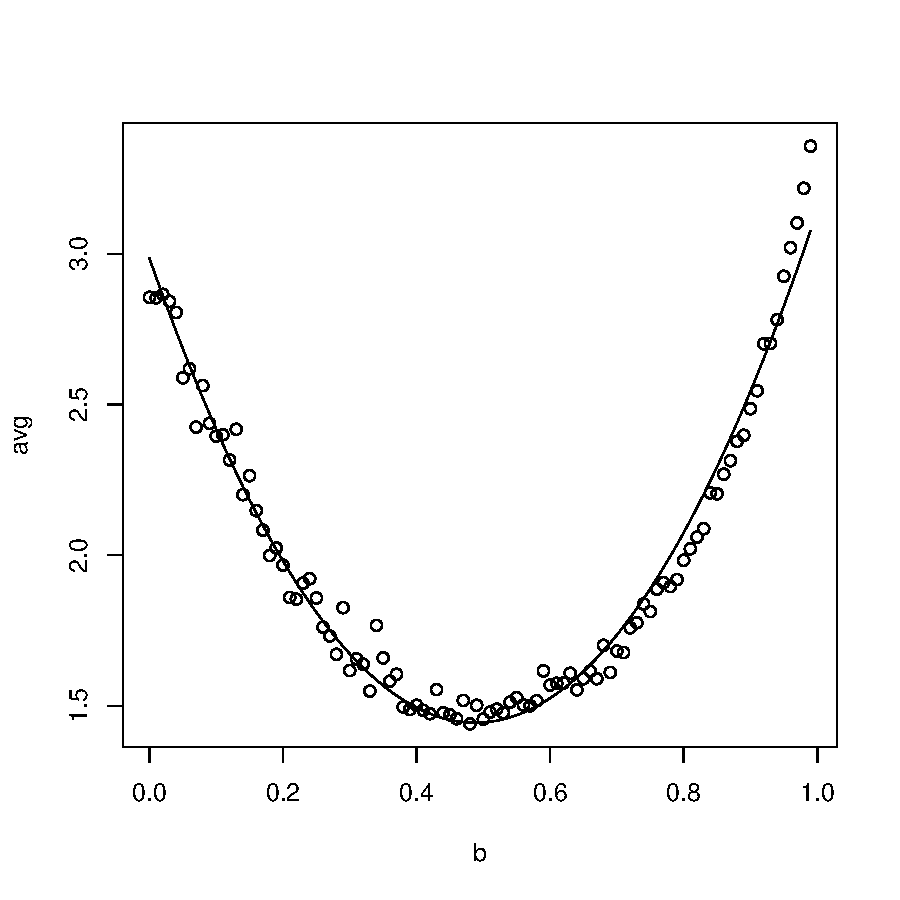
\includegraphics[width=5.0in]{Aloha2.pdf}
}
\caption{Quadratic Curve Superimposed}
\label{qc}
\end{figure}

By the way, even though (\ref{quad}) is a nonlinear function of {\bf b},
it is linear in the $\alpha_i$.  But there are also situations in which
a model which is nonlinear in the parameters is useful.

The most famous of these is the {\bf logistic} model, for the case in
which $Y$ takes on only the values 0 and 1.  As we saw in Section
\ref{propcis}, in this case the expected value becomes a probability.
The logistic model for a nonvector $X$ is then

\begin{equation}
P(Y = 1 | X = t) = \frac{1}{1+e^{\beta_0+\beta_1 t}}
\end{equation}

It extends to the case of vector-valued $X$ in the obvious way. 

The logistic model is quite widely used, especially in medicine,
economics and psychology.

\subsubsection{Nonparametric Estimation of Regression Functions}

What if there is no obvious parametric model for $m_{Yl;X}$?  This is
often the case.  How do we estimate the regression function in such
situations?

To guide our intuition on this, let's turn again of the Davis example of
the relationship between height and weight.  Consider estimation of the
quantity $m_{W;H}(68.2)$, the {\it population} mean weight of all people
of height 68.2.  We could take our estimate $\hat{m}_{W;H}(68.2)$ to be
the average weight of all the people in our sample who have that height.
But we may have very few people of that height, so that our estimate may
have a high variance, i.e. may not be very accurate.

What we could do instead is to take the mean weight of all the people in
our sample whose heights are {\it near} 68.2, say between 67.7 and 68.7.
That would bias things a bit, but we'd get a lower variance.  All
nonparametric regression methods work like this, though with many
variations.

One such method is called {\bf LOESS}.  We won't discuss the details
here, but it basically amounts to estimating $m_{W;H}(68.2)$ via a
complicated process that relies mainly on people in the sample whose
heights are near 68.2.  The R function {\bf lowess()}\footnote{Note the
spelling difference.} implements this method.  I haven't shown it here,
but its result was similar to the fitted parametric model in Figure
\ref{qc}.  

\subsubsection{Assessing Fit of Parametric Model}

Figure \ref{qc} is confirmation that the parametric model was pretty
good.  Visually it seems to fit the scatter plot of the data well.

In this case, in estimating $m_{Y;X}(t)$, $X$ was not vector-valued,
i.e. we had only one ``predictor'' variable.  If we had several
predictor values, e.g. estimating $A$ by {\bf b}, {\bf q} and {\bf s}
(so that ``X'' is a three-component vector), we couldn't draw that
picture so well.  There are other ways to assess the fit of the model,
but we won't go into them here.  Consult any book on statistical
regression analysis.

\subsection{Density Estimation} 

Consider the Bus Paradox example again.  Recall that $W$ denoted the
time until the next bus arrives.  This is called the {\bf forward
recurrence time}.  The {\bf backward recurrence time} is the time since
the last bus was here, which we will denote by $R$.  

Suppose we are interested in estimating the density of $R$, $f_R()$,
based on our sample data from the simulation, $R_1,...,R_n$, where n =
1000 in our example above.  How can we do this?

\subsubsection{Nonparametric Estimation}

Recall that 

\begin{equation}
f_R(t) = \frac{d}{dt} F_R(t) =  \frac{d}{dt} P(R \leq t)
\end{equation}

From calculus, that means that

\begin{eqnarray}
\label{diffquot}
f_R(t) &\approx& \frac{P(R \leq t+h) - P(R \leq t-h)}{2h} \\
&=& \frac{P(t-h < R \leq t+h)}{2h}
\end{eqnarray}

if h is small.  We can then form an estimate $\hat{f}_t(t)$ by plugging
in sample analogs in the right-hand side of (\ref{diffquot}):

\begin{equation}
\label{prehisto}
\hat{f}_R(t) \approx \frac{\#(t-h,t+h))}{2hn} 
\end{equation}

where the notation $\#(a,b)$ means the number of $R_i$ in the interval
(a,b).

There is an important issue of how to choose the value of h here, but
let's postpone that for a minute.  For the moment, let's take 

\begin{equation}
h = \frac{\max_i R_i - \min_iR_i}{100}
\end{equation}

That breaks the interval 

\begin{equation}
\label{hint}
(\min_iR_i, \max_i R_i )
\end{equation}

into 100 subintervals.  

At this point, we'd then compute (\ref{prehisto}) at lots of different
points.  

Although it seems that we must compute (\ref{prehisto}) at infinitely
many values of t, the graph of the function is actually a step function.
Imagine t moving to the right, starting at $\min_iR_i$.  The interval
$t-h,t+h$ moves along with it.  Whenever the interval moves enough to
the right to either pick up a new $R_i$ or lose one that it had had,  
(\ref{prehisto}) will change value, but not at any other time.  So, we
only need to evaluate the function at about $2n$ values of t.

If for some reason we really want to save on computation, let's say that
we compute (\ref{prehisto}) only at the midpoints of the subintervals
(\ref{hint}), and then pretend that the graph of $\hat{f}_R(t)$ is
constant within each subinterval.  Do you know what we get from that?  A
histogram!  Yes, a histogram is a form of density estimation.

Let's see how this works with our Bus Paradox simulation.  We'll use R's
{\bf hist()} to draw some histograms.  First, here's our simulation
code:

\begin{Verbatim}[fontsize=\relsize{-2},numbers=left]
# Bus6.py, illustration of the bus paradox

import random,sys

class glbs:  # globals
   rnd = random.Random(12345)
   lastbus = None  # time last bus arrived
   thisbus = None  # time current bus arrived

def doexpt(opt):
   glbs.lastbus = 0.0
   glbs.thisbus = glbs.rnd.expovariate(0.1)
   while glbs.thisbus < opt:
      glbs.lastbus = glbs.thisbus
      glbs.thisbus += glbs.rnd.expovariate(0.1)
   return 

def main():
   observationpoint = float(sys.argv[1])
   nreps = int(sys.argv[2])
   print 'r'  # to be redirected to a file
   for i in range(nreps):
      doexpt(observationpoint)
      print observationpoint-glbs.lastbus  # to be redirected to a file

if __name__ == '__main__': main()
\end{Verbatim}

I ran this with {\bf nreps} = 1000, and with (as before) {\bf
observationpoint} = 90.  I then ran {\bf hist(r,breaks=100)}, which
specifies 100 subintervals (called {\bf bins} in histogram terminology).
The graph is shown in Figure \ref{h1}.

\begin{figure}[tb] 
\centerline{
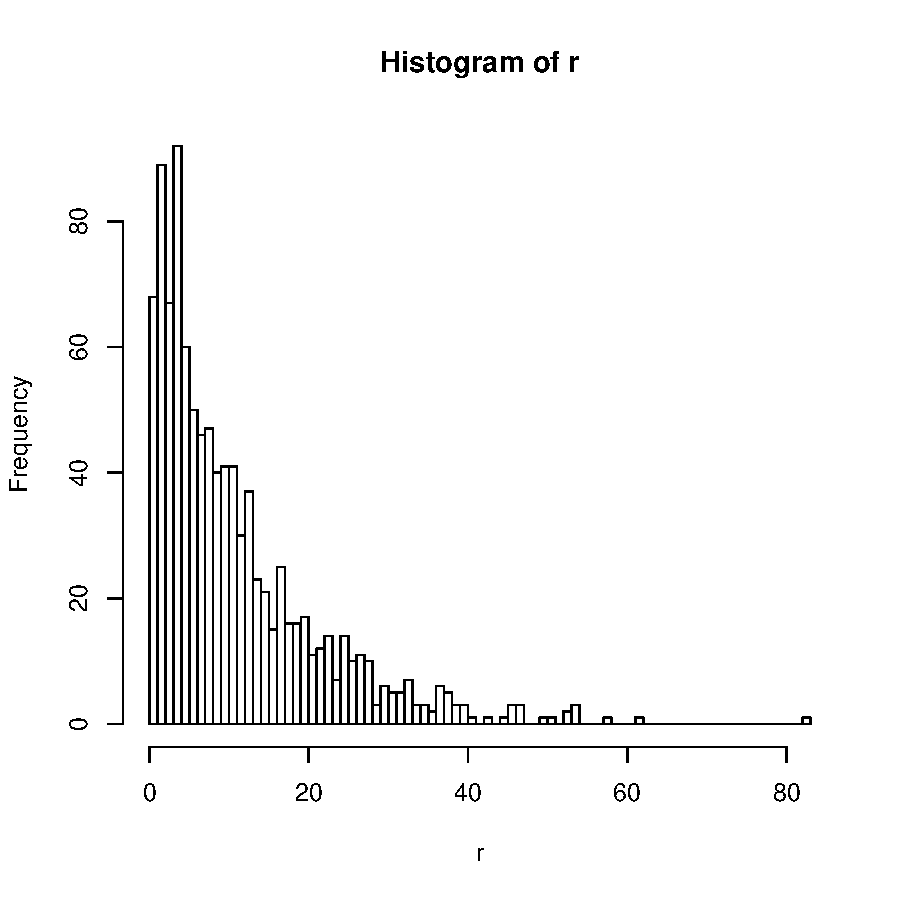
\includegraphics[width=4.0in]{Hist1.pdf} 
}
\caption{Histogram, 100 bins}
\label{h1} 
\end{figure}

This is interesting.  The density seems to have a shape like that of the
gamma family, maybe even exponential (which is a member of the gamma
family).  But 100 bins may be too much for a sample size of 1000, so I
tried 25 bins, shown in Figure \ref{h2}

\begin{figure}[tb] 
\centerline{
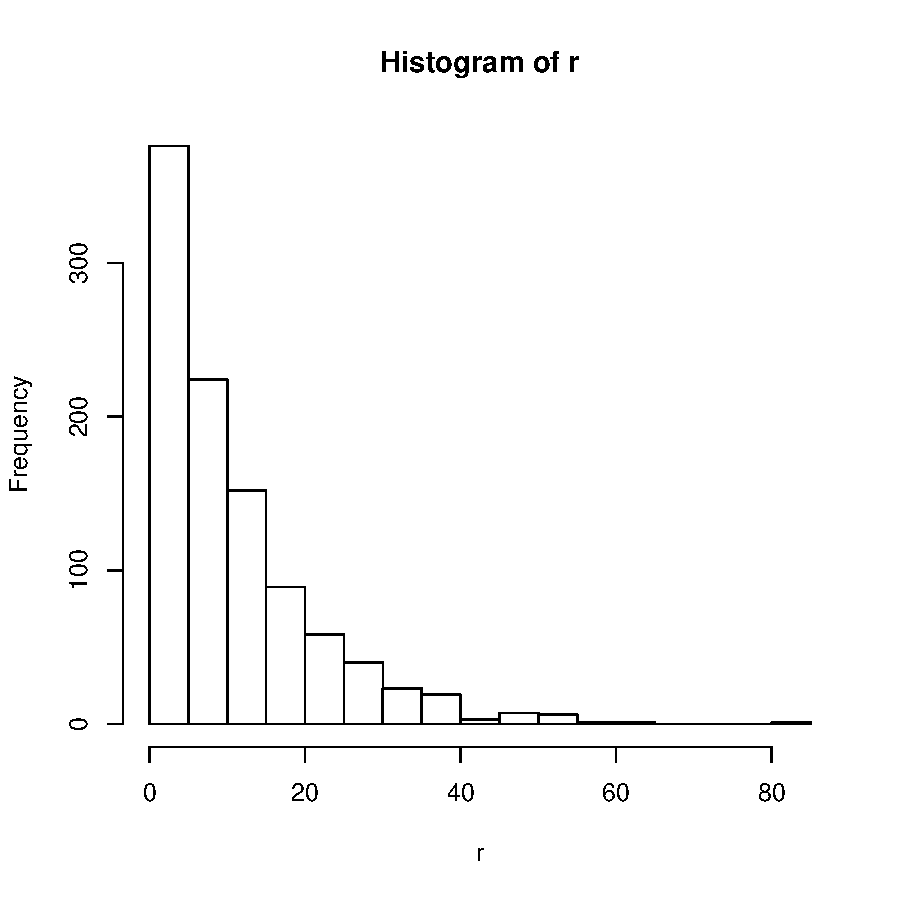
\includegraphics[width=4.0in]{Hist2.pdf}
}
\caption{Histogram, 25 bins}
\label{h2} 
\end{figure}

This illustrates the tradeoff with histograms.  The wider bin width
produces a graph which looks more like a ``curve,'' but with more
oscillation than the true population curve has.

No matter what the bin width is, the histogram will consist of a bunch
of rectanges, rather than a curve.  This is due to the ``quantized''
nature of (\ref{prehisto}):  As the interval (t-h,t+h) moves to the
right, it abruptly gains or loses points.  We could get a smoother
result if we used all points but put more weight on the ones closer to
t.  One way to do this is called {\bf kernel-based} density estimation,
which in R is handled by the function {\bf density()}.  

Kernel estimates also have some similar to our parameter h above,
often called the {\bf bandwidth} (but often denoted by h).  Let's try
the default value, using the call

\begin{Verbatim}[fontsize=\relsize{-2}]
plot(density(r))
\end{Verbatim}

The result is seen in Figure \ref{h3}. 

\begin{figure}[tb] 
\centerline{
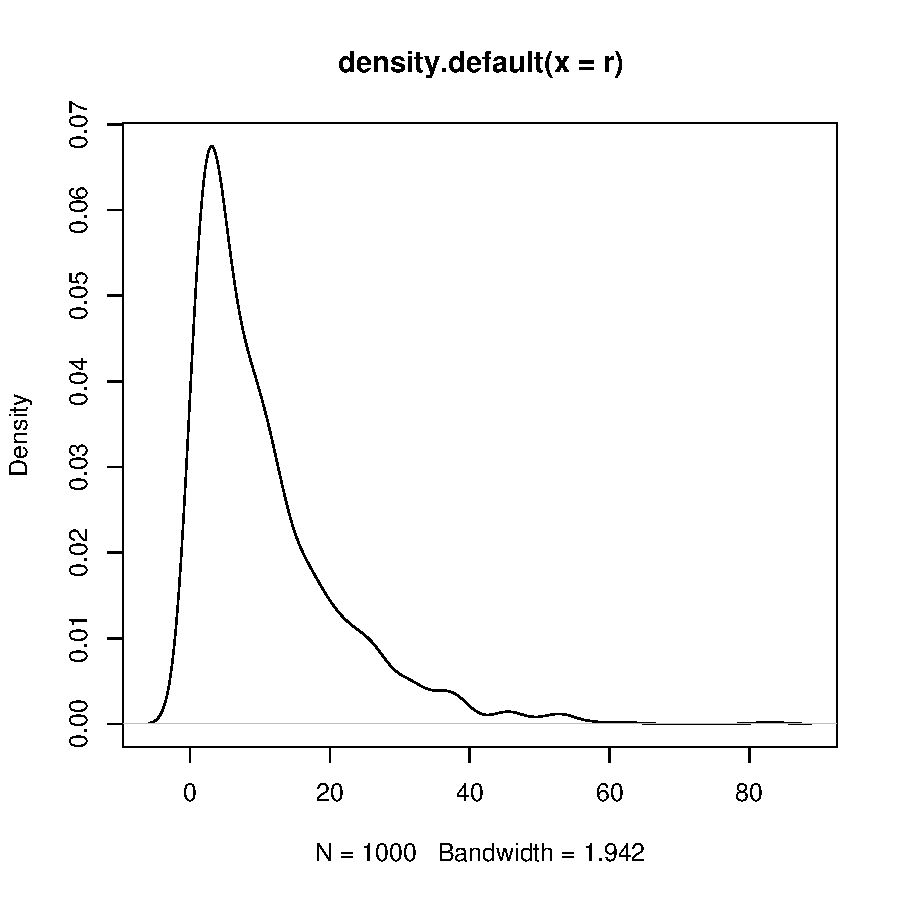
\includegraphics[width=4.0in]{Hist3.pdf} 
}
\caption{Kernel estimate, default bandwidth}
\label{h3}  
\end{figure}

\begin{figure}[tb] 
\centerline{
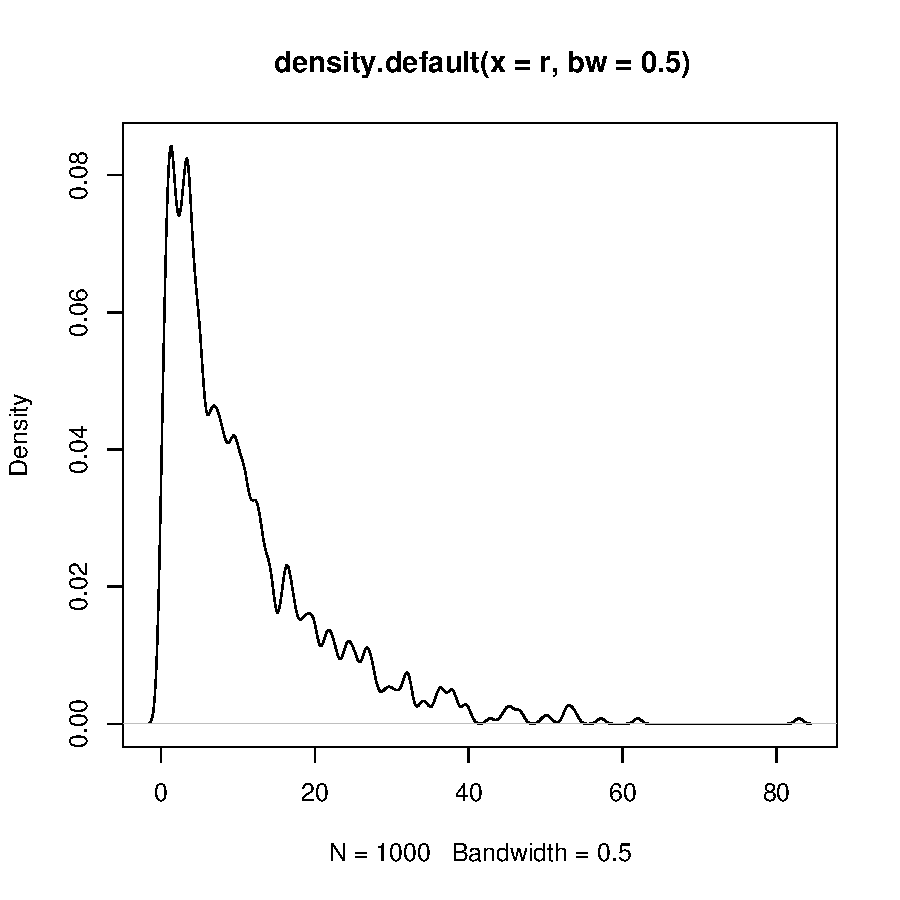
\includegraphics[width=4.0in]{Hist4.pdf}
}
\caption{Kernel estimate, bandwidth 0.5}
\label{h4}   
\end{figure}

I then tried it with a bandwidth of 0.5.  See Figure \ref{h4}.  This
curve oscillates a lot, so 0.5 is probably too small.

Those of you who are reading this in the U.S. or Asia will probably find
the above discussion troubling, as there is no single exact answer to
the problem.  But that's real life!  The question is how to use that
exploratory analysis in a meaningful way.

Even though there is a lot of theory to suggest how to choose the bin
width in histograms and the bandwidth in kernel estimates, no method is
foolproof.  But all in all, the figures suggest a gamma density, maybe
even an exponential.  Note that the density does not necessarily belong
to any parametric family; we are merely exploring whether some
parametric family is a suitable model, i.e. close to the density $f_R$.

\subsubsection{Parametric Estimation}

If we have decided that $f_R$ is well approximated by a certain
parametric family, we can estimate the curve that way.

In our case here, our nonparametric exploration suggested that $f_R$ may
be modeled by the gamma family.  Our model would be

\begin{equation}
\label{gamma}
f_R(t) = \frac{1}{\Gamma(c)} \lambda^t t^{c-1} e^{-\lambda t}, ~ t > 0
\end{equation}

for some $c$ and $\lambda$.  Recall that the parametric model
(\ref{par}), if reasonable, would simplify our estimation of the
regression curve from infinitely many values down to just two values, c
and d.  The situation is similar here; instead of estimating the value
of $f_R$ at infinitely values of t, we need estimate only two values,
$c$ and $\lambda$.

How might we estimate those two parameters?  The most famous way is the
{\bf Method of Maximum Likelihood}.  But that would be rather complex
here, so let's use the {\bf Method of Moments}, as follows.

We know from our previous unit that the gamma distribution has mean
$c/\lambda$ and variance $c/\lambda^2$.  So we set these quantities
equal to their sample values, $\bar{R}$ and $s^2$:

\begin{equation}
\frac{\hat{c}}{\hat{\lambda}} = \bar{R}
\end{equation}

\begin{equation}
\frac{\hat{c}}{\hat{\lambda} ^ 2} = s^2
\end{equation}

Dividing the two quantities yields

\begin{equation}
\hat{\lambda} = \frac{\bar{R}}{s^2}
\end{equation}

which then gives

\begin{equation}
\hat{c} = \frac{\bar{R}}{s^2}
\end{equation}

Of course, our code to calculate $\bar{R}$ and $s^2$ would be like

\begin{Verbatim}[fontsize=\relsize{-2},numbers=left]
   ...
   for i in range(nreps):
      doexpt(observationpoint)
      r = observationpoint-glbs.lastbus
      sum += r
      sum2 += r*r
   rbar = sum/nreps
   s2 = sum2/nreps - rbar**2
   ...
\end{Verbatim}

We would then plug these into (\ref{gamma}), and that would be our
estimated density.

\subsubsection{Assessing Fit of Parametric Model}

If we did fit a gamma model above, we would like to check it.

You have probably studied statistical hypothesis testing, and may have
seen the {\bf Chi-Squared Goodness of Fit Test}, which could be used
here.  The null hypothesis would be that $f_R$ is exactly equal to some
member of the gamma family.

{\bf Don't use hypothesis testing, either for simulation output or any
other application!}  In the simulation case, we generate such a large
sample that we are almost sure to reject the null hypothesis---even if 
the null hypothesis is ``approximately true.''  For instance, our
density $f_R$ above might be very close to a gamma density, close enough
for our purpose, but with a large enough sample our test will tell us
not to use the model.

This is true in nonsimulation applications as well.  With a large
sample, your test will pounce on small, meaningless deviations from the
null hypotheses.  Very small samples won't be able to detect interesting
deviations.  For any given application, it's hard to determine whether
the sample size is large enough.  

Even if you overcome these problems, a test will still never give you as
much information as a confidence interval will.

For assessing model fit for a density, you can form a {\bf
Kolmogorov-Smirnov confidence band}, which works as follows.

Recall that $F_R$ denotes the cdf of $R$.  Define its sample analog,
called the {\bf empirical distribution function}, by

\begin{equation}
\hat{F}_R(t) = \frac{\#(-\infty,t)}{n}
\end{equation}

In the bus problem, say we store the $R_i$ in a list {\bf r}, and then
sort it, naming the values in the sorted array $Y_i$.  Then
$\hat{F}_R(t)$ would be 0 for $-\infty < t < Y_1$, it would be 1/n for
$Y_1 < t < Y_2$, and so on.

To make a 95\% confidence band for $F_R$, we add and subtract
$1.36/\sqrt{n}$ to $\hat{F}_R(t)$ at all values of t.  If some member of
the gamma family fits into that band, or comes close enough, then we
would decide the gamma fit to be a good one.

\subsubsection{Oh, By the Way}

It can be proven that the distribution of $R$ really is exponential.

\section{Statistical Inference in Infinite Time Horizon Settings}

\subsection{Illustrative Example}

Recall our ALOHA network example in Section \ref{regintro}.  Let $Y_i$
denote the number of active nodes at epoch i.  There we were interested
in time 8, i.e. in $\nu_8 = E(Y_8)$.  In many other situations, we may
be interested instead in what happens as time goes to infinity.  But
what does that really mean?

Intuitively, we feel that this system will converge to steady state in
some sense.  This certainly doesn't mean in the deterministic sense.
The latter would mean

\begin{equation}
\lim_{i \rightarrow \infty} Y_i
\end{equation}

which cannot be true; the $Y_i$ will continue to fluctuate.  But we do
feel that they will have a long-run average, i.e. that

\begin{equation}
\label{cesaro}
\lim_{i \rightarrow \infty} \frac{Y_1+...+Y_i}{i}
\end{equation}

will exist as some constant $\nu$ and that 

\begin{equation}
\label{nulim}
\lim_{i \rightarrow \infty} E(Y_i) = \nu
\end{equation}

These things can be proven under certain reasonable mathematical
conditions.  In fact, under these conditions one can show that 

\begin{equation}
\lim_{i \rightarrow} F_{Y_i}(t)
\end{equation}

exists for each t.  That sounds pretty abstract, but here it simply
means that

\begin{equation}
\label{pyik}
\lim_{i \rightarrow} P(Y_i = k)
\end{equation}

exists for each k.  For instance, the probability that there are, say, 3
nodes active at time i will converge as i gets large.

The questions of interest here will be

\begin{itemize}

\item How long do we need to run the simulation to get a reasonably
accurate estimate of $\nu$?

\item How can we find a valid confidence interval for $\nu$?

\end{itemize} 

\subsection{Mathematical Statement of the Problem}

This task would be straightforward in the case of estimating $\nu_8$.
We could simulate, say, 1000 replications of the system through time 8.
Letting $Y_{8j}$ denote the $j^{th}$ of these replications, we would
these random variables would be {\it independent} and {\it identically
distributed} with mean $\nu_8$.  Equation (\ref{meanci}) would apply
perfectly.  The width of the confidence interval would then give us a
good idea as to the accuracy of our estimate of $\nu$.

The situation in (\ref{cesaro}) is not nearly so straightforward.  There
the $Y_i$ are {\it neither} independent {\it nor} identically
distributed.  Let's look at this a bit more:

\begin{itemize} 

\item The $Y_i$ are not independent.  The number of nodes at time 28,
say, will have some effect on the number at time 29.

\item The $Y_i$ are not identically distributed.  The process does
converge to a steady state, but each it has a different distribution at
each finite time.  For example, $Y_1 = 0$ with certainty, while $\lim_{i
\rightarrow} P(Y_i = 0)$ will be quite different.

\end{itemize}

The key to (\ref{meanci}) was not just the Central Limit Theorem but
also the facts that 

\begin{equation}
\label{unbmean}
E(\bar{W}) = \frac{1}{n} E(W_1+...+W_n) = \frac{1}{n}
[E(W_1)+...+E(W_n)] = \frac{1}{n} \cdot n \mu = \mu
\end{equation}

and

\begin{equation}
\label{addvar}
Var(\bar{W}) = \frac{1}{n^2} Var(W_1+...+W_n) = \frac{1}{n^2}
[Var(W_1)+...+Var(W_n)] = \frac{1}{n^2} \cdot n \sigma^2 =
\sigma^2/n
\end{equation}

In our case now, the fact that the $Y_i$ are not identically
distributed is reflected in

\begin{equation}
\label{biased}
E(Y_i) \neq \nu
\end{equation}

The fact that the $Y_i$ are not independent is reflected in

\begin{equation}
Var(Y_1+...+Y_n) = Var(Y_1)+...+Var(Y_n) + 2 \sum_{r \neq s}
Cov(Y_r,Y_s) \neq Var(Y_1)+...+Var(Y_n)
\end{equation}

The problem of not being identically distributed can be phrased as
saying that near the beginning of the simulation, we are in a {\bf
transient period}, during which the process is settling down to steady
state.  Of course, technically speaking, the transient period is
infinite, since we ``reach'' steady state only after an infinite amount
of time.  But in practical terms, we come reasonably close enough to
steady state after a finite amount of time.  In (\ref{pyik}), for
instance, the limiting probability for k = 2 might be, say, 0.64, but
after a certain number of epochs it will be within 0.02 of that.

Similarly, due to (\ref{nulim}), we see that (\ref{biased}) is not so
much of an issue after some number of epochs.

\subsection{Determining the Transient Period}

The problem of the $Y_i$ not being identically distributed is somewhat
easier to deal with.  To discuss that, let's start by looking at
(\ref{cesaro}): 

\begin{Verbatim}[fontsize=\relsize{-2},numbers=left]
# AlohaC2.py, form of slotted ALOHA

import random, sys 

class node:  # one object of this class models one network node
   s = 4  # number of nodes
   b = 0.3  # backoff parameter; refrain from sending with probability b
   q = 0.2  # msg creation probability
   activeset = []  # which nodes are active now
   inactiveset = []  # which nodes are inactive now
   r = random.Random(98765)  
   def __init__(self):  
      node.inactiveset.append(self)
   def checkgoactive():  # generate nodes which change to active
      for n in node.inactiveset:
         if node.r.uniform(0,1) < node.q:
            node.inactiveset.remove(n)
            node.activeset.append(n)
   checkgoactive = staticmethod(checkgoactive)  
   def trysend():  # the active nodes try to send, or not
      numnodestried = 0  
      whotriedlast = None  
      for n in node.activeset:
         if node.r.uniform(0,1) > node.b:
            whotriedlast = n
            numnodestried += 1
      if numnodestried == 1:
         node.activeset.remove(whotriedlast)
         node.inactiveset.append(whotriedlast)
   trysend = staticmethod(trysend)  
   def reset():  
      for n in node.activeset:
         node.activeset.remove(n)
         node.inactiveset.append(n)
   reset = staticmethod(reset)  
            
def main():
   for i in range(node.s): node()
   sum = 0  
   for epoch in range(10000):  # simulate until time 9999
      node.checkgoactive()
      node.trysend()
      sum += len(node.activeset)  # add Yi to total
      print epoch, float(sum)/(epoch+1)  # to be redirected to a file

if __name__ == '__main__': main()
\end{Verbatim}

Here we've adapted the program to look only at a specific value of {\bf
b}, and to look at many epochs instead of replications for epoch 8.
Most importantly, we are printing out the values of (\ref{cesaro}) as we
go along.  Figure \ref{meanyi} shows the graph of these values. 

\begin{figure}[tb]
\centerline{
% 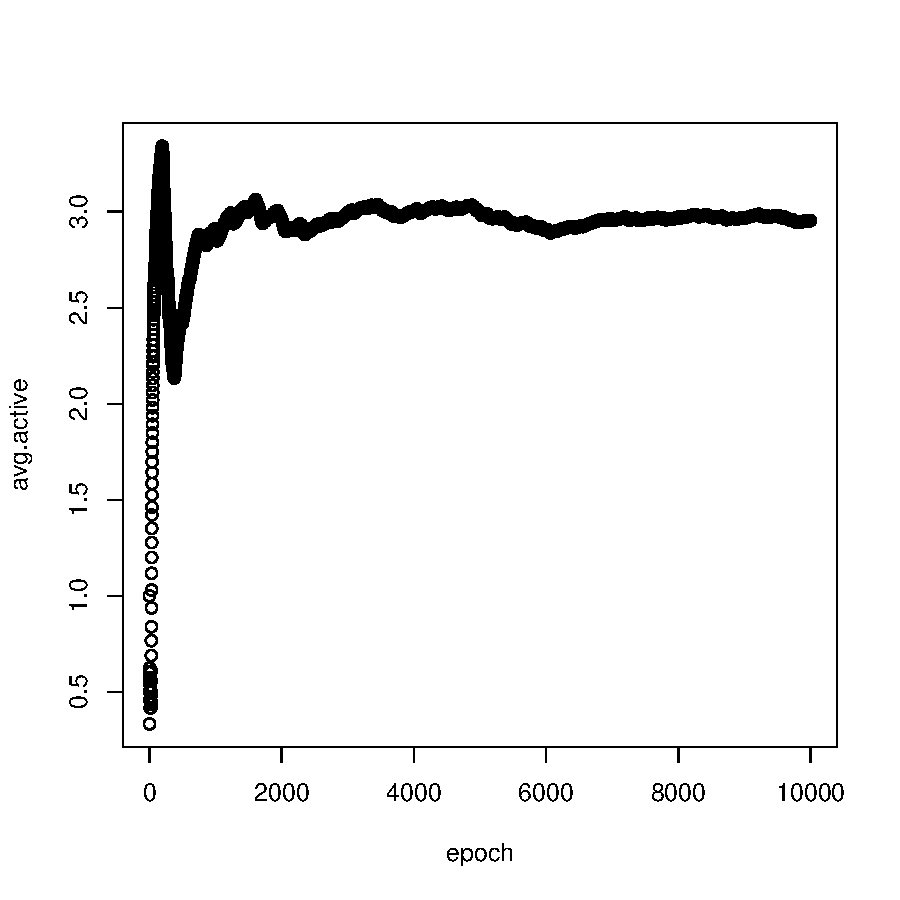
\includegraphics[width=4.0in]{Cesaro2.pdf}
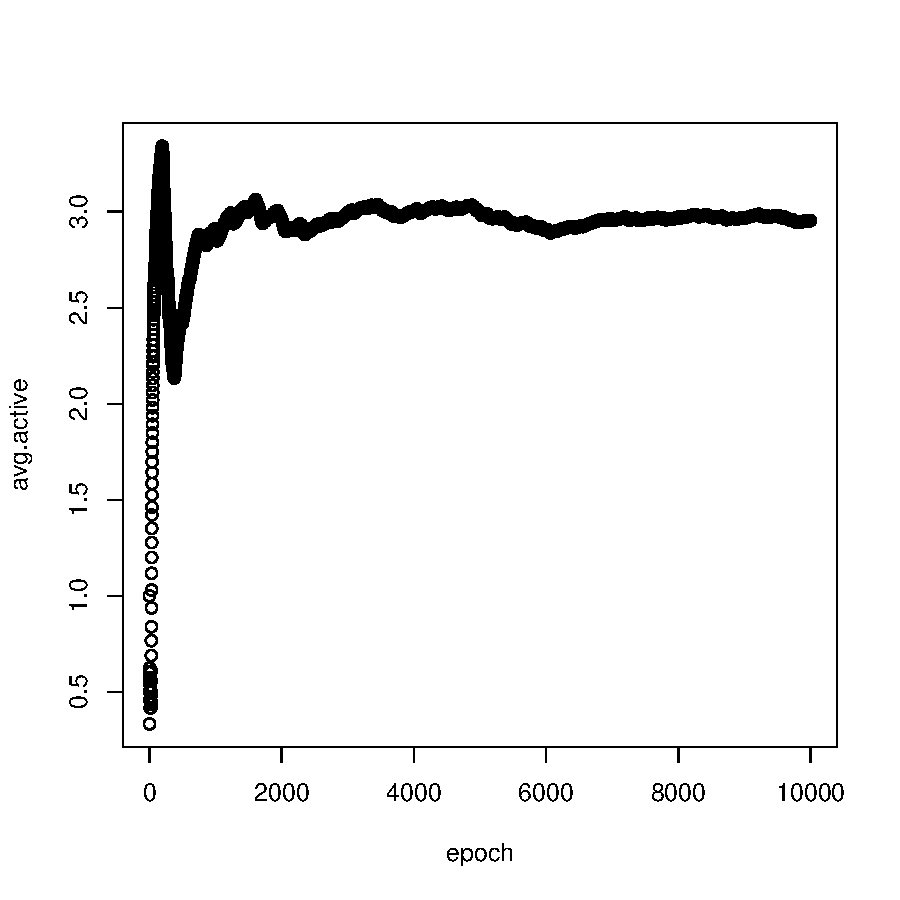
\includegraphics{Cesaro2.pdf}
}
\caption{Mean Yi}
\label{meanyi}
\end{figure}

Convergence seems to occur after about 1000 epochs.  What that says is
that to deal with the problem of (\ref{biased}), we can just throw out
the first 1000 epochs of our simulation.  Instead of computing

\begin{equation}
\label{ces1}
\frac{Y_1+...+Y_{10000}}{10000}
\end{equation}

we would compute

\begin{equation}
\label{ces2}
\frac{Y_{1001}+...+Y_{10000}}{9000}
\end{equation}

Actually, even discarding 1000 observation is much too conservative.
The expected values in (\ref{nulim}) converge much faster than that.
The slowness of convergence here is due to the fact that we have only
one observation at each epoch.  If we were to do many replications at
each epoch (i.e.  run the above code, with 10000 epochs, in many
replications), we'd see much faster convergence.  Short of doing that,
though, we can take the conservative route.

\subsection{Has the Simulation Run Long Enough?}

We see that (\ref{cesaro}) has settled down to around 2.95.  For
informal purposes, this may be good enough.

But in many applications of simulation we must present not only the
sample estimate but also a margin of error.  So, again we must ask how
to find a confidence inteval for $\nu$.

\subsection{Confidence Intervals}

We saw above how to deal with the fact that our observations $Y_i$ are
not identically distributed.  What should we do about their lack of
independence?  There are three main methods for handling this, which we
will now describe.

\subsubsection{The Replications Method}

Here we would run, say, 1000 replications of the simulation up to time
10000, getting 1000 values of (\ref{ces2}).  These values would be
independent and identically distributed, and thus we could form a
confidence interval for $\nu$ using (\ref{meanci}).

This is a clean way to solve the problem, but obviously with
considerable extra run time.

\subsubsection{The Batch Means Method}

Though our $Y_i$ are not independent, they are approximately independent
when spaced far enough apart.  For instance, $Y_{26}$ and $Y_{39}$
should have almost nothing to do with each other.

So, we could take our 9000 observations $Y_{1001},...,Y_{10000}$ and
divide them into batches of size, say, 50.  $Y_{1001},...,Y_{1050}$
would be the first batch, $Y_{1051},...,Y_{1100}$ would be the second
batch, and so on.  Let $B_k$ denote the mean Y value in the $k^{th}$
batch.  Then the $B_k$ would be approximately independent, by virtue of
the spacing, and approximately identically distributed, by virtue of
their having occurred past the transient period.  Thus we could use them
in (\ref{meanci}), with 9000/50 = 180 in place of n,
$\sum_{k=1}^{180}B_k/180$ in place of $\bar{W}$, and with s calculated
from (\ref{s2}) for the $B_k$. 

This is probably the most common method.

\subsubsection{The Regenerative Process Method}

This method is the most elegant of the three, though it is not always
practical.

The key to this method is to find a state of the system in which ``time
starts over.''  This is similar in concept to the memoryless property of
the exponential distribution family, and in fact we'll see later a
connection.

Let's again illustrate this with our ALOHA example.  Our network starts
out with zero nodes active.  After some random amount of time, we will
again have zero nodes active.  Then this number will become nonzero for
another random amount of time before returning to zero again.  The
process will repeatedly go through these cycles.  

The point is that each time we start a new cycle, ``time starts over,''
since the subsequent behavior of the network doesn't depend on what
happened before we reached state 0.  If we were to compute the average
value of Y in each of these cycles, these averages would thus be
independent and identically distributed, which could be used in
(\ref{meanci}).  This idea, with a bit of refinement, is the basis of
the regenerative method.

To explain the details, consider an example from our introductory unit
on SimPy, at
\url{http://heather.cs.ucdavis.edu/~matloff/156/PLN/DESimIntro.pdf}.  We
have two machines, whose up times are exponentially distributed with
intensity 1.0, and whose repair times are exponentially distributed with
intensity 0.5.  The repairperson is not summoned until both machines are
down.  We are interested in the proportion $\rho$ of the time in which
both machines are up simultaneously.

Consider the times at which the system enters the state in which both
machines are up, which we will call the ``full capacity state.''  Our
simulation has them start in this state.  After a while, one of the
machines will go down, then the other.  Then one of the machines, say
machine B, will begin repair, and after that is done, the other machine,
A, will begin repair.  Say B does not go down again before A's repair
ends.  When the latter event occurs we have entered into the full
capacity state for the second time.

We must first ask the question, does ``time start over'' at that time?
Probabilistically speaking, is the distribution of the process from that
time onward the same as it was starting at time 0.0?  The answer is yes,
but only because up times are exponentially distributed and thus
memoryless.  If up times were to have some other distribution, then when
A comes up, B would be either more likely or less likely to fail in the
upcoming moments than it was a time 0.0.  So, without the exponential
distribution here, time would NOT ``start over'' when A comes up.

But if up times are exponentially distributed, the times at which we
enter the full capacity state do indeed delineate periods in which the
system acts independently and with the same
distribution.\footnote{\label{indp}Note that we have also tacitly
assumed that the two machines act independently of each other, that for
a given machine its successive up times are independent and so on.} We
call these times {\bf regeneration points}.

There are other sets of regeneration points in this process as well.
One such set consists of the times at which the repairperson is
summoned.  This set is especially important, because it does not depend
on the assumption of exponential distributions.\footnote{It does
continue to depend on the independence assumptions mentioned in footnote
\ref{indp}.} So, we'll use this one for our example.

Let $T_i$ denote the $i^{th}$ time the repairperson is summoned, i =
1,2,...  Assume we start the simulation in that state too, and thus set
$T_0 = 0.0$.  This breaks time into a series of regeneration cycles.
Let $D_i = T_i - T_{i-1}$ represent the duration of the $i^{th}$ cycle.
We run the simulation for n cycles.

Remember, we are interested in finding $\rho$, the proportion of the
time in which both machines are up simultaneously.  To that end, 
let $C_i$ denote the total amount of time the system is in full capacity
during the $i^{th}$ cycle.  It can be proved, and it is intuitive, that 

\begin{equation}
\label{iglehart}
\rho = \frac{E(C)}{E(D)}
\end{equation}

where $C$ and $D$ are random variables having the common distribution of
the $C_i$ and $D_i$, respectively.  Then the natural estimate of $\rho$
based on our simulation output is

\begin{equation}
\hat{\rho} =
\frac
{\overline{C}}  % \bar{} wasn't showing up well, so used \overline{}
{\overline{D}}
= 
\frac
{\sum_{i=1}^{n} C_i}
{\sum_{i=1}^{n} D_i}
\end{equation}

Now consider the random variables $X_i = C_i - \rho D_i$.  Remember, we
don't know the value of $\rho$, but these random variables exist.  

Because of the nature of the regeneration cycles, the $X_i$ are
independent and identically distributed.  From (\ref{iglehart}), we know
that they have mean 0.  

Thus the Central Limit Theorem (CLT) tells us that the random variables

\begin{equation}
\label{regenclt}
\frac
{\overline{X}}
{\sqrt{Var(X)/n}}
\end{equation}

are approximately distributed N(0,1) when n is large.  

For a generic random variable $X$ having the distribution of the $X_i$,

\begin{equation}
\label{varcov}
Var(X) = Var(C) + \rho^2 Var(D) - 2\rho Cov(C,D)
\end{equation}

We can replace by sample analogs in (\ref{regenclt}) and still have the
CLT hold.  In other words, the quantity

\begin{equation}
\label{regenclt2}
\frac
{\overline{X}}
{s_X/n^{0.5}}
\end{equation}

has an approximate N(0,1) distribution, where $s_X$ is our sample-based
estimate of the standard deviation of X, obtained by taking sample
analogs in (\ref{varcov}):  

\begin{equation}
s^2_X = \frac{1}{n} \sum_{i=1}^n (C_i - \bar{C})^2 +
\hat{\rho}^2  \frac{1}{n} \sum_{i=1}^n (D_i - \bar{D})^2 -
2 \hat{\rho} \frac{1}{n} \sum_{i=1}^n (C_i - \bar{C}) (D_i - \bar{D})
\end{equation}

After some algebra (not shown here), we then find that an approximate
95\% confidence interval for $\rho$ is

\begin{equation}
\label{rhoci}
(\hat{\rho} - 1.96 \frac{s_X}{\overline{D} n^{0.5}},
\hat{\rho} + 1.96 \frac{s_X}{\overline{D} n^{0.5}})
\end{equation}

Now, how does this generalize to other systems?  Let $V_t$ denote the
state of our system at time t.  $V_t$ is a vector of quantities that
fully describe the current state of the system.  For instance, in our
machine repair example above, $V_t$ would consist of the following
quantities at time t:

\begin{itemize}

\item 1 or 0, according to whether machine A is up 

\item 1 or 0, according to whether machine B is up 

\item time A has been up, if it's up

\item time B has been up, if it's up

\item 1 or 0, according to whether machine A is being repaired 

\item 1 or 0, according to whether machine B is being repaired 

\item time A has been under repair, if it's been repaired

\item time B has been under repair, if it's being repaired

\end{itemize}

We need that the population quantity $\gamma$ that we are trying to
estimate be of the form 

\begin{equation}
\label{gammalim}
\gamma = \lim_{t \rightarrow \infty} \frac{1}{t} \int_{0}^{t} h(V_u) ~ du
\end{equation}

for some function h.  In our machine repair example we had

\begin{equation} 
h(t) = \begin{cases} 
   1, & \text{if full capacity at time t} \\ 
   0, & \text{otherwise} \\ 
\end{cases} 
\end{equation}

Here, the integral in (\ref{gammalim}) is the total time we are in full
capacity during (0,t).  Dividing that integral by t gives us the
proportion of time we are in full capacity during (0,t).

In a queuing system simulation, if we are interested in the long-run
average queue length, $h(V_t)$ would simply be the length of the queue
at time t.  In this case, its integral from 0 to t is the sum of the
queue lengths during that time, multiplied by the amount of time each length
occurred.

Then to an approximate 95\% confidence for $\gamma$ would be
(\ref{rhoci}), where now

\begin{equation}
C_i = \int_{T_{i-1}}^{T_i} h(V_u) ~ du
\end{equation}

and 

\begin{equation}
\label{gammahat}
\hat{\gamma} = \frac{1}{T_n} \int_{0}^{T_n} h(V_u) ~ du
\end{equation}

For instance, in the queuing example, (\ref{gammahat}) would be the
average queue length during our simulation, where again this would mean
a weighted average in which the weights are the times that the queue
length has been at the various values.

Note that in a simulation with a very complicated state vector, a
regeneration point may be difficult to find.  Moreover, the regeneration
cycles may be extremely long.  These considerations make this method
difficult to use in some applications. 

